%!TEX root = ../../thesis.tex

The \ggHWW analysis is binned according to jet multiplicity, in order to exploit the vastly 
different background compositions in each jet bin (see \Figure~\ref{fig:sel:njets}); the 
0-jet, 1-jet and \twojet bins each have dedicated event selection criteria. Uncertainties 
in the expected ggF cross section must be evaluated separately for each jet bin, and 
correlations considered when the bins are combined. Perturbative uncertainties in the jet 
binning itself are considered independently from the other selection criteria, since they 
posses some additional subtleties.



\subsection{Perturbative uncertainties in jet-binned cross sections}
\label{sec:ggF:naive}

Consider splitting a cross section into two parts: an exclusive 0-jet cross section, 
$\sigma_0$, and an inclusive $\geq\!1$-jet cross section, $\sigma_{\geq1}$:
\begin{equation}
	\sigma_{\total} = \sigma_0 \parenths{\ptcut} + \sigma_{\geq1} \parenths{\ptcut}
\end{equation}
where \ptcut is the jet \pt threshold \cite{YR2}. In $\sigma_{\geq1}$, the requirement of 
a jet with $\pt > \ptcut$ introduces double logarithmic contributions 
$\alpha_{\text{S}}^{k+m} L^{2m}$, where $L \sim \ln\parenths{\ptcut/Q}$ and $Q$ is the 
scale of the hard scatter ($Q = \mH$ for ggF). These terms are analogous to the logarithms 
introduced by soft gluon emission (see \Section~\ref{sec:qcd:resum}), though they depend 
upon the process and also the jet algorithm and parameters (\eg \antikt with $R=0.4$).

The schematic structures of the two inclusive cross sections are
\begin{equation}
	\sigma_{\total} &\sim \alpha_{\text{S}}^k \{1 &+& \alphaS &+& \alpha_{\text{S}}^2 &+& \ofOrder{\alpha_{\text{S}}^3}\} \\
	\sigma_{\geq1}  &\sim \alpha_{\text{S}}^k \{&\phantom{{}=+}&\alphaS (L^2 + L + 1) &+& \alpha_{\text{S}}^2 (L^4 + L^3 + L^2 + L + 1) &+& \ofOrder{\alpha_{\text{S}}^3 L^6}\} \,.
\end{equation}
When $\ptcut \ll \mH$, the logarithms can overcome the \alphaS suppression and provide 
significant corrections to $\sigma_{\geq1}$. When similar in size to the perturbative 
corrections to $\sigma_{\total}$, the scale dependence of $\sigma_0 = \sigma_{\total} - 
\sigma_{\geq1}$ is reduced by cancellations between the two series. This suggests that 
na\"{i}vely varying \mur and \muf might underestimate perturbative uncertainties. This is 
confirmed by \Figure~\ref{fig:ggF:naive}, which shows that the cancellations at 
\unit{$\ptcut = 25$}{\GeV} (used in the \HWW analysis) are rather extreme.

\begin{figure}[t]
	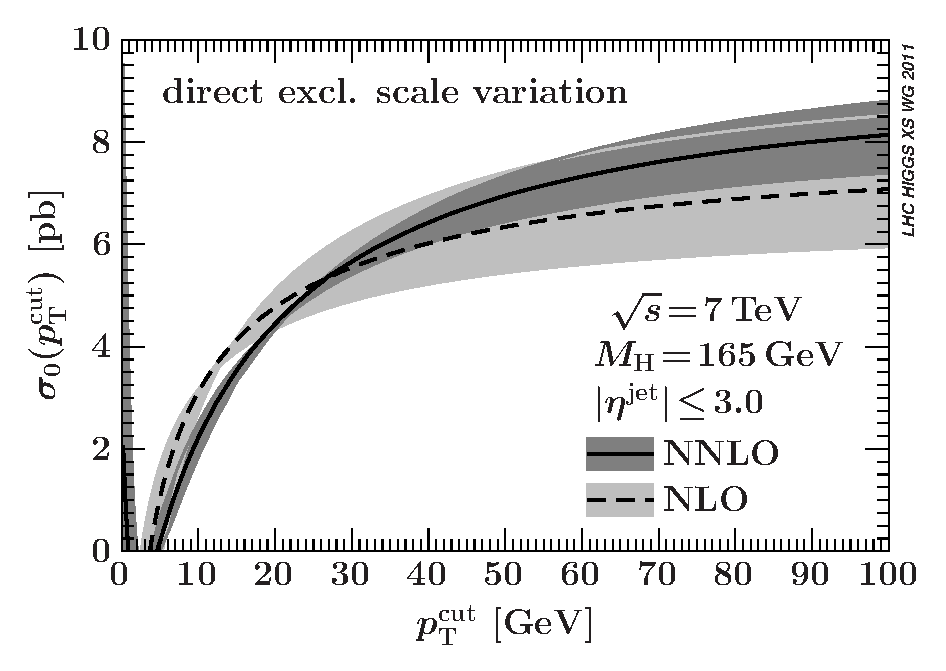
\includegraphics[width=\mediumfigwidth]{tex/signal/sigma0_naive}
	\caption{The exclusive 0-jet ggF cross section versus the jet \pt threshold \cite{YR2}. 
	The band shows the perturbative uncertainties evaluated via na\"{i}ve scale variations.}
	\label{fig:ggF:naive}
\end{figure}

When discussing uncertainties in jet-binned cross sections, it is convenient to consider 
a general parametrisation of the covariance matrix. In the \braces{\sigma_0, \sigma_{\geq1}}
basis, the covariance matrix is decomposed into two uncertainty sources
\begin{equation}
	C &= C^{\text{yield}} + C^{\text{migration}} \\
	&= \twomatrix{\parenths{\Delta^{\text{y}}_0}^2 & \Delta^{\text{y}}_0 \Delta^{\text{y}}_{\geq1}}{\Delta^{\text{y}}_0 \Delta^{\text{y}}_{\geq1} & \parenths{\Delta^{\text{y}}_{\geq1}}^2} + \parenths{\Delta_{0\rightarrow}^{\text{mig}}}^2\twomatrix{1 & -1}{-1 & 1} \,.
\end{equation}
The yield component is fully correlated between jet bins, though can affect them with 
different magnitudes. The migration component is fully anti-correlated and affects both 
bins equally, conserving the normalisation. In the limit setting procedure, these sources 
are treated as nuisance parameters with \braces{\sigma_0, \sigma_{\geq1}} uncertainty 
amplitudes
\begin{equation}
	\begin{array}{l@{}l@{}l}
		\begin{array}{r}
			\kappa^{\text{yield}}              : \Big( \\
			\kappa^{\text{mig}}_{0\rightarrow} : \Big(
		\end{array}
		&
		\begin{array}{@{}rrr@{}}
			\Delta^{\text{y}}_0, & \Delta^{\text{y}}_{\geq1} \\
			\Delta^{\text{mig}}_{0\rightarrow}, & -\Delta^{\text{mig}}_{0\rightarrow}
		\end{array}
		&
		\begin{array}{@{}l}
			\Big) \\ \Big) \,.
		\end{array}
	\end{array}
	\label{eq:ggF:2bin_np}
\end{equation}

Different prescriptions for evaluating perturbative uncertainties are defined by their 
choice of $\Delta^{\text{y}}_0$, $\Delta^{\text{y}}_{\geq1}$ and 
$\Delta^{\text{mig}}_{0\rightarrow}$. This includes a choice of observables to measure 
uncertainties in, and also the method of measuring the uncertainties. For example, the 
na\"{i}ve prescription described above is equivalent to choosing
\begin{equation}
	\text{Na\"{i}ve:} 
	\quad\quad \Delta^{\text{y}}_0 &= \Delta\sigma_{0},& 
	\quad\quad \Delta^{\text{y}}_{\geq1} &= \Delta\sigma_{\geq1},&
	\quad\quad \Delta^{\text{mig}}_{0\rightarrow} &= 0
\end{equation}
where uncertainties are evaluated at fixed order by varying \mur and \muf.

In the \HWW analysis, there is also an exclusive 1-jet bin. The second jet veto introduces 
an additional source of migrations, now between the 1-jet and \twojet bins. 
Therefore, in the \braces{\sigma_0, \sigma_1, \sigma_{\geq2}} basis, the covariance 
matrix has three components
\begin{equation}
	C &= 
	\threematrix{
		\parenths{\Delta^{\text{y}}_0}^2 & 
		\Delta^{\text{y}}_0 \Delta^{\text{y}}_1 & 
		\Delta^{\text{y}}_0 \Delta^{\text{y}}_{\geq2}
	}{
		\Delta^{\text{y}}_0 \Delta^{\text{y}}_1 & 
		\parenths{\Delta^{\text{y}}_1}^2 & 
		\Delta^{\text{y}}_1 \Delta^{\text{y}}_{\geq2}
	}{
		\Delta^{\text{y}}_0 \Delta^{\text{y}}_{\geq2} & 
		\Delta^{\text{y}}_1 \Delta^{\text{y}}_{\geq2} & 
		\parenths{\Delta^{\text{y}}_{\geq2}}^2
	}
	\nonumber \\
	&+ \parenths{\Delta^{\text{mig}}_{0\rightarrow}}^2
	\threematrix{
		1 & -\parenths{1-\rho} & -\rho
	}{
		-\parenths{1-\rho} & \parenths{1-\rho}^2 & \rho\parenths{1-\rho}
	}{
		-\rho & \rho\parenths{1-\rho} & \rho^2
	}
	+ \parenths{\Delta^{\text{mig}}_{1\rightarrow}}^2
	\threematrix{
		0 & 0 & 0
	}{
		0 & 1 & -1
	}{
		0 & -1 & 1
	}
\end{equation}
where $\rho$ is the fraction of migrations from the 0-jet bin that enter the \twojet bin. 
In this case, there are three nuisance parameters with uncertainty amplitudes
\begin{equation}
	\begin{array}{l@{}l@{}l}
		\begin{array}{r}
			\kappa^{\text{yield}}              : \Big( \\
			\kappa^{\text{mig}}_{0\rightarrow} : \Big( \\
			\kappa^{\text{mig}}_{1\rightarrow} : \Big(
		\end{array}
		&
		\begin{array}{@{}rrr@{}}
			\Delta^{\text{y}}_0, & \Delta^{\text{y}}_1, & \Delta^{\text{y}}_{\geq2} \\
			\Delta^{\text{mig}}_{0\rightarrow}, & -\parenths{1-\rho} \Delta^{\text{mig}}_{0\rightarrow}, & -\rho \Delta^{\text{mig}}_{0\rightarrow} \\
			0, & \Delta^{\text{mig}}_{1\rightarrow}, & -\Delta^{\text{mig}}_{1\rightarrow}
		\end{array}
		&
		\begin{array}{l}
			\Big) \\ \Big) \\ \Big) \,.
		\end{array}
	\end{array}
	\label{eq:ggF:3bin_np}
\end{equation}
So it is $\Delta^{\text{y}}_0$, $\Delta^{\text{y}}_1$, $\Delta^{\text{y}}_{\geq2}$, 
$\Delta^{\text{mig}}_{0\rightarrow}$, $\Delta^{\text{mig}}_{1\rightarrow}$ and $\rho$ 
that must be determined. Two different prescriptions for evaluating these shall now be 
examined.



\subsection{Combined inclusive prescription}
\label{sec:ggF:ci}

The \textit{combined inclusive} (CI) prescription\footnote{
	The CI prescription is also called the Stewart-Tackmann prescription, after its 
	original proponents.
} \cite{Stewart-Tackmann:2012} uses scale variations of $\sigma_{\geq1}$ and 
$\sigma_{\geq2}$ to probe the size of the higher order logarithmic corrections, and 
identifies that they are related to the bin migration uncertainties. It therefore chooses
\begin{equation}
	\text{CI:}
	\quad\quad \Delta^{\text{y}}_0 &= \Delta\sigma_{\total},&
	\quad\quad \Delta^{\text{y}}_1 &= 0,&
	\quad\quad \Delta^{\text{y}}_{\geq2} &= 0, \nonumber \\
	\quad\quad \Delta^{\text{mig}}_{0\rightarrow} &= \Delta\sigma_{\geq1},&
	\quad\quad \Delta^{\text{mig}}_{1\rightarrow} &= \Delta\sigma_{\geq2},&
	\quad\quad \rho &= 0
\end{equation}
where $\Delta\sigma_{\total}$, $\Delta\sigma_{\geq1}$ and $\Delta\sigma_{\geq2}$ are 
evaluated at fixed order by varying \mur and \muf.

This is equivalent to assuming inclusive cross sections have uncorrelated uncertainties
\begin{equation}
	\text{CI:} \quad\quad
	\sigma_N = \sigma_{\geq N} - \sigma_{\geq N+1}
	\quad\quad\Rightarrow\quad\quad
	\Delta\sigma_N^2 = \Delta\sigma_{\geq N}^2 + \Delta\sigma_{\geq N+1}^2 \,.
\end{equation}
Although this assumption is not believed to be exact, the CI prescription offers a 
practical solution to the cancellations described in \Section~\ref{sec:ggF:naive} (see 
\Figure~\ref{fig:ggF:ci}). It ensures that uncertainties in exclusive cross sections are 
larger than those in the corresponding inclusive cross section, \ie $\Delta\sigma_{N} \geq 
\Delta\sigma_{\geq N}$, and the large-\ptcut limit agrees with expectations. 

\begin{figure}[t]
	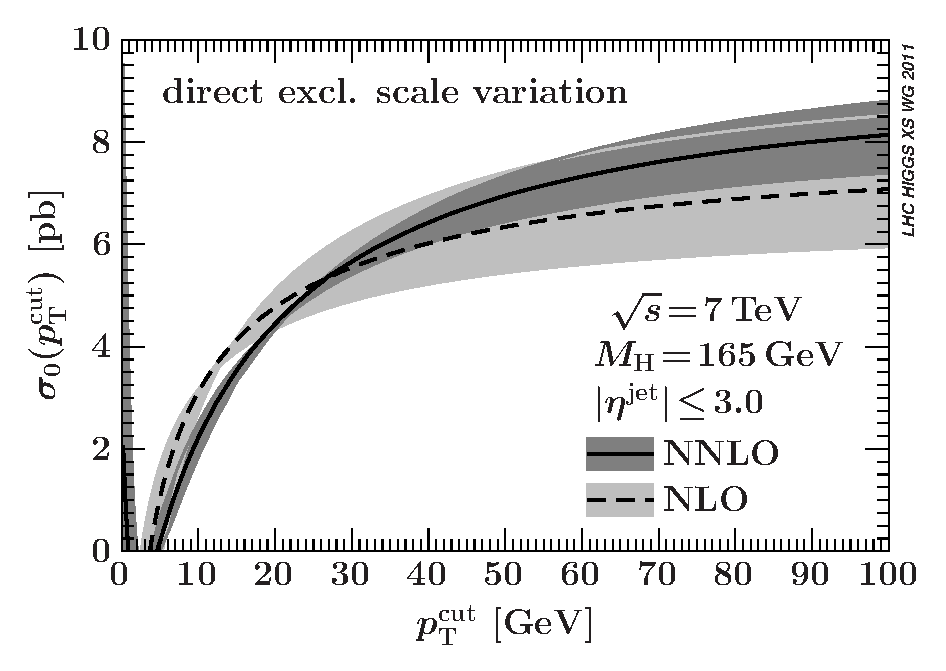
\includegraphics[width=0.495\textwidth]{tex/signal/sigma0_naive}
	\hfill
	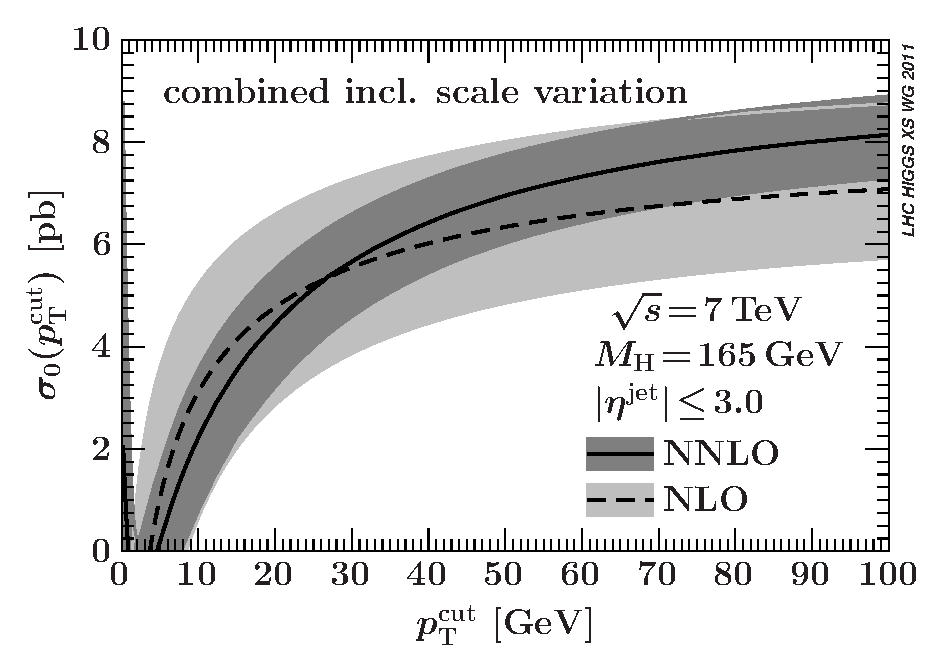
\includegraphics[width=0.495\textwidth]{tex/signal/sigma0_CI}
	\caption{The exclusive 0-jet ggF cross section versus the jet \pt threshold 
	\cite{YR2}. The band shows the perturbative uncertainties evaluated using the 
	na\"{i}ve prescription (left) and the combined inclusive prescription (right).}
	\label{fig:ggF:ci}
\end{figure}

It should be emphasised that each inclusive cross section must be evaluated at the same 
order in \alphaS (\eg $\sigma_{\total}^{\text{NNLO}}$, $\sigma_{\geq1}^{\text{NLO}}$ and 
$\sigma_{\geq2}^{\text{LO}}$). This can restrict the application of the CI prescription. 
For example, an exclusive 2-jet bin cannot be added until $\sigma_{\total}$ is calculated 
at NNNLO in QCD. For the ggF contamination to the VBF signal region (defined with a central 
jet veto), $\sigma_{\geq2}^{\text{NLO}}$ and $\sigma_{\geq3}^{\text{LO}}$ can be used since 
they are evaluated in a significantly different phase space 
($\Delta\sigma_{\geq2}^{\text{NLO}}$ and $\Delta\sigma_{\geq2}^{\text{LO}}$ are treated as 
fully correlated).

\hnnlo \cite{HNNLO} is used to compute $\sigma_{\total}^{\text{NNLO}}$, 
$\sigma_{\geq1}^{\text{NLO}}$ and $\sigma_{\geq2}^{\text{LO}}$. However, the CI 
prescription can be improved by using the NNLO+NNLL(QCD)+NLO(EW) $\sigma_{\total}$ 
calculation \cite{YR3}, which has smaller perturbative uncertainties than 
$\sigma_{\total}^{\text{NNLO}}$. In order to combine these results whilst preserving the 
total normalisation, the jet bin fractions $f_N = \sigma_N/\sigma_{\total}$ from \hnnlo are 
used to propagate the $\Delta\sigma_{\geq N}$ to $\Delta\sigma_{N}$:
\begin{equation}
	\delta\sigma_0^2 &= \frac{1}{f_0^2}\delta\sigma_{\total}^2 + \parenths{\frac{1}{f_0}-1}^{\!\!2}\delta\sigma_{\geq1}^2 \label{eq:ggF:ci_1} \\
	\delta\sigma_1^2 &= \parenths{\frac{1-f_0}{f_1}}^{\!\!2}\delta\sigma_{\geq1}^2 + \parenths{\frac{1-f_0}{f_1}-1}^{\!\!2}\delta\sigma_{\geq2}^2 \label{eq:ggF:ci_2}
\end{equation}
where $\delta\sigma_i = \Delta\sigma_i/\sigma_i$. This assumes the uncertainties are 
Gaussian distributed, though the nuisance parameters are implemented as log-normal 
distributions in the fitting code. The $\Delta\sigma_{\geq N}$ are evaluated via 
independent variation of \mur and \muf in the range $\mH/4 \leq \mur,\muf \leq \mH$, whilst 
observing the constraint $1/2 \leq \mur/\muf \leq 2$. These are then propagated to 
$\Delta\sigma_N$ using (\ref{eq:ggF:ci_1}) and (\ref{eq:ggF:ci_2}), as shown in 
\Table~\ref{tab:ggF:ci}.

\begin{table}
	\begin{tabular}{r@{\hskip 0.3in}c@{\hskip 0.3in}r@{\hskip 0.3in}r}
		\toprule
		\multicolumn{1}{c@{\hskip 0.3in}}{$i$} & $f_i = \sigma_i/\sigma_{\total}$ & \multicolumn{1}{c@{\hskip 0.3in}}{$\sigma_i$ (\pico\barn)} & \multicolumn{1}{c}{$\Delta\sigma_i/\sigma_i$} \\
		\midrule
		$\geq\!0$ & --    & 19.27 &  7.8\% \\
		$\geq\!1$ & --    & \multicolumn{1}{c@{\hskip 0.3in}}{--} & 20.2\% \\
		$\geq\!2$ & --    & \multicolumn{1}{c@{\hskip 0.3in}}{--} & 69.7\% \\
		\midrule
		\cline{3-4}
		$0$       & 0.614 & \multicolumn{1}{|r@{\hskip 0.3in}}{11.83} & \multicolumn{1}{r|}{18.0\%} \\
		$1$       & 0.267 &  \multicolumn{1}{|r@{\hskip 0.3in}}{5.15} & \multicolumn{1}{r|}{42.6\%} \\
		$\geq\!2$ & --    &  \multicolumn{1}{|r@{\hskip 0.3in}}{2.29} & \multicolumn{1}{r|}{69.7\%} \\
		\cline{3-4}
		\bottomrule
	\end{tabular}
	\caption{Inputs and outputs (boxed) of the combined inclusive prescription for ggF, 
	with \unit{$\mH = 125$}{\GeV} and \unit{$\sqrt{s} = 8$}{\TeV}. All inputs computed by 
	\hnnlo except $\sigma_{\total}$ and $\Delta\sigma_{\total}$, which are from 
	\Reference~\cite{YR3}.}
	\label{tab:ggF:ci}
\end{table}




\subsection{Jet veto efficiency method}
\label{sec:ggF:jve}

The \textit{jet veto efficiency} (JVE) method \cite{JVE:NLL} takes quite a different 
approach. It considers each exclusive cross section as a product of the total cross 
section and jet veto efficiencies
\begin{equation}
	\sigma_0 &= \sigma_{\total} \epsilon_0 \\
	\sigma_1 &= \sigma_{\total} \parenths{1-\epsilon_0} \epsilon_1 \\
	\sigma_{\geq2} &= \sigma_{\total} \parenths{1-\epsilon_0} \parenths{1-\epsilon_1}
\end{equation}
where $\epsilon_0 = \epsilon_0\parenths{\ptcut}$ and 
$\epsilon_1 = \epsilon_1\parenths{p_{\text{T}}^{\text{sel}}, \ptcut}$ are the first and 
second jet veto efficiencies. It then assumes that uncertainties in $\sigma_{\total}$ and 
$\epsilon_N$ are uncorrelated, and therefore exclusive cross sections must have an 
uncertainty at least as large as $\Delta\sigma_{\total}$. This is equivalent to
\begin{equation}
	\text{JVE:}
	\quad\quad \Delta^{\text{y}}_0 &= \Delta\sigma_{\total} \, \frac{\sigma_{0}}{\sigma_{\total}} \,,&
	\quad\quad \Delta^{\text{y}}_1 &= \Delta\sigma_{\total} \, \frac{\sigma_{1}}{\sigma_{\total}} \,,&
	\quad\quad \Delta^{\text{y}}_{\geq2} &= \Delta\sigma_{\total} \, \frac{\sigma_{\geq2}}{\sigma_{\total}} \,, \nonumber \\
	\quad\quad \Delta^{\text{mig}}_{0\rightarrow} &= \Delta\epsilon_0 \, \sigma_{\total} \,,&
	\quad\quad \Delta^{\text{mig}}_{1\rightarrow} &= \Delta\epsilon_1 \, \sigma_{\geq1} \,,&
	\quad\quad \rho &= 1-\epsilon_1 \,.
\end{equation}
Again, $\Delta\sigma_{\total}$ is taken from \Section~\ref{sec:ggf_inc}. However, 
$\epsilon_N$ contains similar cancellations to those discussed in 
\Section~\ref{sec:ggF:naive}, and so $\Delta\epsilon_N$ must be treated with care.

There is an ambiguity in the definition of $\epsilon_N$ that is not present in fixed 
order calculations. For example, at NNLO, three alternative definitions of 
$\epsilon_N$ may be identified
\begin{equation}
	\epsilon_N^{\parenths{\text{a}}} &= 1 - \frac{\sigma_{\geq N+1}^{\text{NLO}}}{\sigma_{\geq N}^{\text{NNLO}}} \\
	\epsilon_N^{\parenths{\text{b}}} &= 1 - \frac{\sigma_{\geq N+1}^{\text{NLO}}}{\sigma_{\geq N}^{\text{NLO}}} \\
	\epsilon_N^{\parenths{\text{c}}} &= 1 - \frac{\sigma_{\geq N+1}^{\text{NLO}}}{\sigma_{\geq N}^{\text{LO}}} + \parenths{\frac{\sigma_{\geq N}^{\text{NLO}}}{\sigma_{\geq N}^{\text{LO}}} - 1} \frac{\sigma_{\geq N+1}^{\text{LO}}}{\sigma_{\geq N}^{\text{LO}}} \,.
\end{equation}
Schemes (a), (b) and (c) differ by N$^3$LO terms, and therefore can probe higher 
order corrections. In processes where convergence is well behaved, \eg 
\HepProcess{\Pquark\APquark \HepTo \PZ}, these schemes converge. Therefore, 
$\epsilon_N^{\parenths{\text{a}}}$ is taken as the central value and $\Delta\epsilon_N$ 
is taken as the difference between the schemes or the scale variations in 
$\epsilon_N^{\parenths{\text{a}}}$, whichever is larger.

\todo[inline]{allows you to improve accuracy of components independently. insert plot showing resummation improvement}


\subsection{Results}

\begin{figure}
	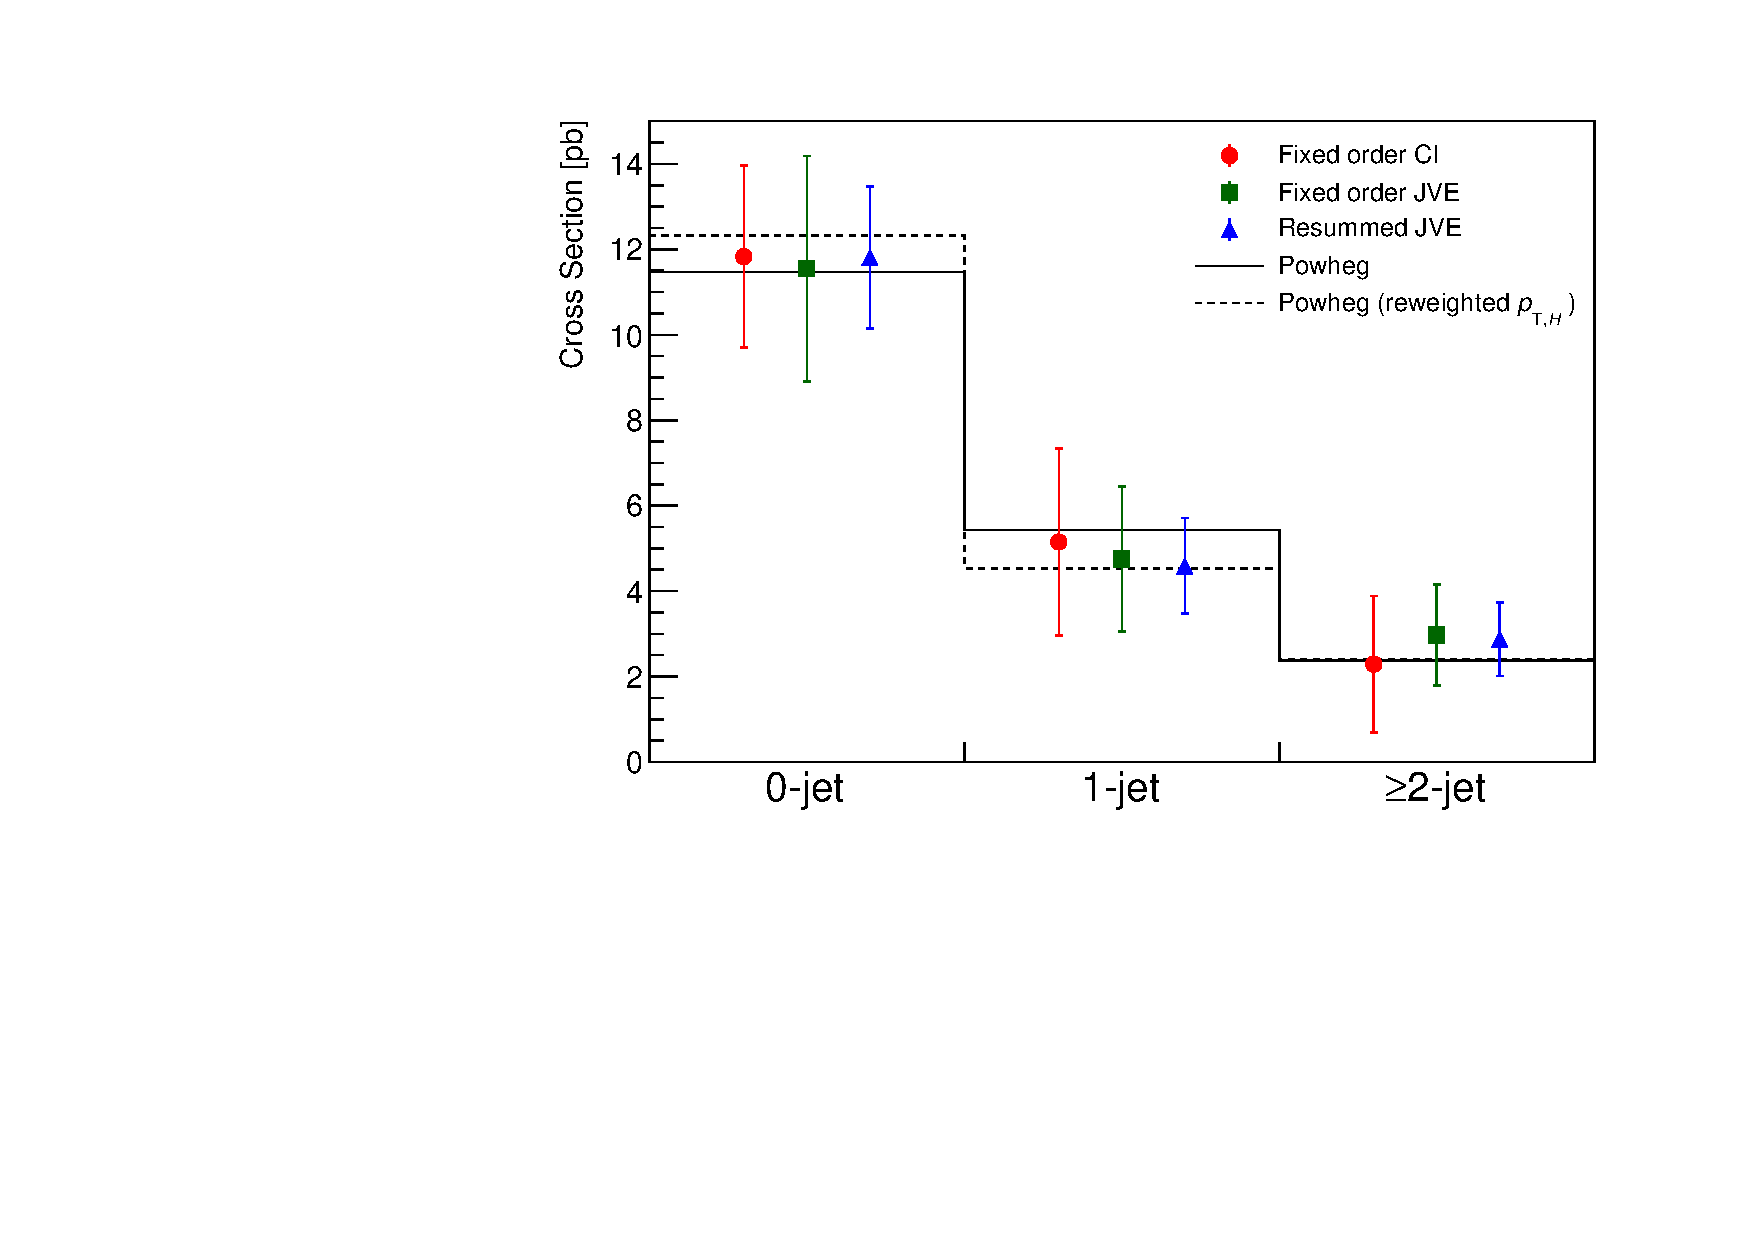
\includegraphics[width=\largefigwidth]{custom_images/ggF_xs_jetbin}
	\caption{Jet-binned cross sections for ggF production with \unit{$\mH = 125$}{\GeV} and 
	\unit{$\sqrt{s} = 8$}{\TeV}. The error bars show the perturbative uncertainty 
	associated with each prescription. Consistency with \meps{\powhegbox}{\pythia{8}} is also shown, normalised to \unit{19.27}{\pico\barn}.}
	\label{fig:signal:jetbin_xs_summary}
\end{figure}
